\section{Présentation du jeu}

SmallCiv est un jeu de stratégie, mélange de Civilization et Small World. Chaque joueur a à sa disposition un certain nombre d'unités, et ces unités lui rapporteront des points à chaque tour en occupant le plus possible de cases sur la carte. Mais elles peuvent également se déplacer ou se battre, et annihiler l'armée adverse est une condition de victoire tout aussi valable. \newline

\begin{figure}
	\centering
	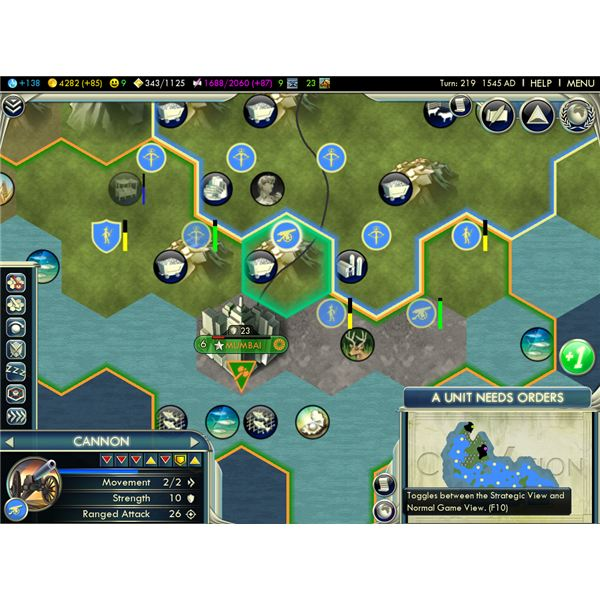
\includegraphics[scale=0.5]{img/map.jpg}
	\caption{Un exemple de carte de Civilization V}
	\label{map}
\end{figure}
Le jeu se déroule sur une carte composée de cases hexagonales (cf. \textsc{figure~\ref{map}}) et se place dans un univers fantastique. L'on retrouvera donc des orcs, des elfes et des nains qui évoluent dans des environnements type plaine ou forêt... Chaque race a ses bonus et malus spécifiques, dont certains sont liés à l'environnement, comme les elfes qui  peuvent se déplacer plus loin en forêt. Les règles du jeu seront détaillées plus en détail dans la partie spécifique. 